%第3章

\section{詳細設計}

オブジェクト間のメッセージのやりとりを時系列に沿って表現するために,以下に示すシーケンス図を作成した.
換気要請についてのシーケンス図を図\ref{sequencekanki}に,室内の監視についてのシーケンス図を図\ref{sequencekanshi}に,室内環境についてのシーケンス図を図\ref{sequenceshitsunai}に,入室危険度についてのシーケンス図を図\ref{sequencenyushitsu}に示す.

\begin{figure}
	\centering
	\includegraphics[width=15cm]{./uml/sequence_kanki_2}
	\caption{換気要請についてのシーケンス図}
	\label{sequencekanki}
\end{figure}

「換気要請」について,まずセンサデバイスが3分経過ごとに二酸化炭素センサへ値の取得指示を出す.
取得した二酸化炭素濃度をJetsonへ送信し,Jetsonはセンサデータベースへデータを記録した後,15分間分のデータをデータベースから取得する.
次にカメラから画像を取得し人数推定を行う.推定した人数と取得した二酸化炭素濃度値を,警戒レベルが保有する上限人数と二酸化炭素濃度の基準値と比較し換気要請の判断を行う.その後換気要請に応じてLEDとブザーに指示を出す.

\begin{figure}
	\centering
	\includegraphics[width=15cm]{uml/sequence_kanshi_3}
	\caption{室内の監視についてのシーケンス図}
	\label{sequencekanshi}
\end{figure}

「室内の監視」について,システムを起動するとJetsonはセンサデバイスへ開始の指示を行う.
指示を受けたセンサデバイスは二酸化炭素センサへ値の取得指示を出す.
その後はセンサデバイスが3分経過ごとに二酸化炭素センサへ値の取得指示を出し,人数推定を行うまで「換気要請」の場合と同様であり,
推定した人数と取得した二酸化炭素濃度値を,警戒レベルが保有する上限人数と二酸化炭素濃度の基準値と比較し,警戒レベルを設定する.

\begin{figure}
	\centering
	\includegraphics[width=15cm]{uml/sequence_shitsunai_2}
	\caption{室内環境についてのシーケンス図}
	\label{sequenceshitsunai}
\end{figure}

「室内環境」について,まずセンサデバイスが3分経過ごとに温湿度センサへ値の取得指示を出す.
取得した温湿度をJetsonへ送信し,Jetsonはセンサデータベースへデータを記録した後,これまでの温湿度データを取得する.
温湿度の平均値を算出し,適正範囲内か否かによって温湿度アラートLEDを制御する.

\begin{figure}[htbp]
\centering
\includegraphics[width=15cm]{./uml/sequence_nyushitsu_e.eps}
\caption{入室危険度についてのシーケンス図}
\label{sequencenyushitsu}
\end{figure}

「入室危険度」について,人数推定を行うまでは「換気要請」等と同様の流れである.
その後,現在の室内滞在人数と,警戒レベルが保有する滞在上限人数,滞在推奨人数を比較し入室危険度を決定する.
Jetsonから室外デバイスに入室危険度を送信し,室外デバイスは入室危険度に応じてLEDの制御を行う.
赤枠で囲んだ屋外デバイスとLEDは筆者が実装を担当する.

次に,筆者が実装を担当した室外デバイスのステートチャート図を図\ref{statechartokugai}に示す.

\begin{figure}
	\centering
	\includegraphics[width=0.3\linewidth]{uml/statechart_okugai_1}
	\caption{室外デバイスのステートチャート図}
	\label{statechartokugai}
\end{figure}

室外デバイスはシステムが稼働している間,常に入室危険度の受信待機状態であり,Jetsonから入室危険度が送られてきた場合に入室危険度に応じた色のLEDが点灯する.

以上の詳細設計より表\ref{tantaitestsitsugaikoumoku}に示す室外デバイスにおける単体テスト項目を挙げた.

\begin{table}
	\centering
	\caption{室外デバイスにおける単体テスト項目}
	\label{tantaitestsitsugaikoumoku}
	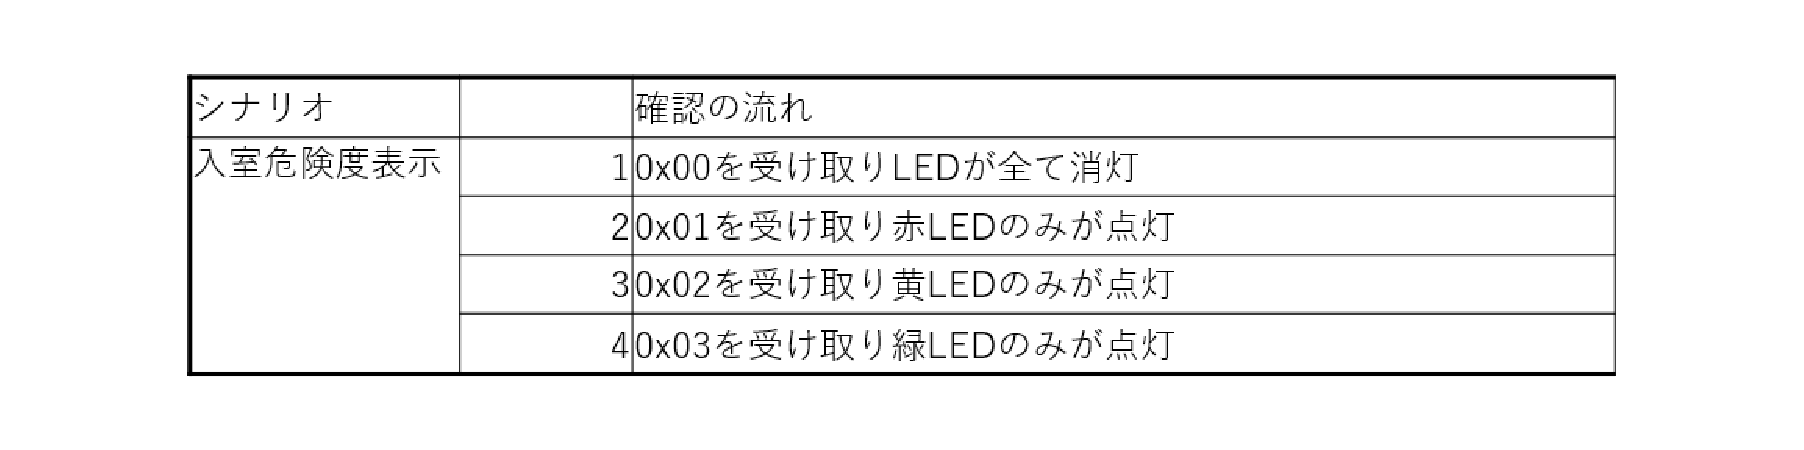
\includegraphics[width=0.9\linewidth]{test/tantaitest_sitsugai_koumoku2}
\end{table}